\documentclass[10pt]{article}

\usepackage[letterpaper]{geometry}
\usepackage{enumerate,verbatim,mdwlist}
\usepackage{fancyhdr}
\usepackage{linguex}
\usepackage[colorlinks=true,linkcolor=blue]{hyperref}

%Packages needed for trees
\usepackage{amsfonts,amsmath,amssymb}
\usepackage[varg]{txfonts}
\usepackage{qtree}
\usepackage{multicol}

%%%%%%%%%%%%%%%%%%%%%%%%%%%%%%%%%%%%%%%%%%%%%
%% Represent categorical logic graphically %%
%%%%%%%%%%%%%%%%%%%%%%%%%%%%%%%%%%%%%%%%%%%%%

\usepackage{tikz}
\usepackage{xstring}

\usetikzlibrary{shapes,backgrounds}
\tikzstyle{every node}=[font=\tiny] 

%%%%%%%%%%%%%%%%%%%%%%%%%%%%%%%%
%% Draw squares of Opposition %%
%%%%%%%%%%%%%%%%%%%%%%%%%%%%%%%%

\def\oppsquare{(-1.5,1) node[above left]{$All$} -- (1.5,1) node[above right]{$No$} -- (1.5,-1) node[below right]{$Some-not$} -- (-1.5,-1) node[below left]{$Some$} -- (-1.5,1)}
\def\oppcross{(-1.5,1) -- (1.5,-1) node[sloped,above,pos=0.3]{contra} node[sloped,above,pos=0.7]{dictory} (-1.5,-1) -- (1.5,1) node[sloped,above,pos=0.3]{contra} node[sloped,above,pos=0.7]{dictory}}

\def\sqroppMod{%
  \begin{scope}
    \draw \oppsquare;
    \draw \oppcross;
    \draw (-1.75,0) node[rotate=90] {undet.};
    \draw (0,1.25) node {undet.};
    \draw (0,-1.25) node {undet.};
    \draw (1.75,0) node[rotate=90] {undet.};
  \end{scope}
}

\def\sqroppTrad{%
  \begin{scope}
    \draw \oppsquare;
    \draw \oppcross;
    \draw (-1.75,0) node[rotate=90] {subalt.};
    \draw (0,1.25) node {contrary};
    \draw (0,-1.25) node {subcontrary};
    \draw (1.75,0) node[rotate=90] {subalt.};
  \end{scope}
}

%%%%%%%%%%% Turn categorical props into Venn diagrams %%%%%%%%%%%%%%%
%% \catvenn{title:<y/n>}{quantifier:<All/No/Some>}{quality:<not/>} %%
%%         {complement:<non-/>}{subject class}                     %%
%%         {complement:<non-/>}{predicate class}                   %%
%%%%%%%%%%%%%%%%%%%%%%%%%%%%%%%%%%%%%%%%%%%%%%%%%%%%%%%%%%%%%%%%%%%%%

%%%%%%%%%%%%%
%% Circles %%
%%%%%%%%%%%%%

%% Venn circles
\def\firstcircle{(0,0) circle (1cm)} 
\def\secondcircle{(0:1.5cm) circle (1cm)}
\def\thirdcircle{(60:1.5cm) circle (1cm)}

%% Overlapping and disjoint circles
\def\firstcircleN{(0,0) circle (.75cm) node [below left=.25in] {$A$}}
\def\secondcircleN{(0:2cm) circle (.75cm) node [below right=.25in] {$B$}}
\def\firstcircleA{(0,0) circle (1.25cm) node [above right] {$A$}}
\def\secondcircleA{(.125,0) circle (.75cm) node [below left=.25in] {$B$}}

%%%%%%%%%%%%%%%%%%%%%%%%%%%
%% Venn diagram template %%
%%%%%%%%%%%%%%%%%%%%%%%%%%%

\newcommand{\vennbox}[2]{%
  \draw (-1.5,-1.5) rectangle (3,1.5);
  \draw \firstcircle node [below left=.25in] {#1};
  \draw \secondcircle node [below right=.25in] {#2};
}

\newcommand{\syllbox}[3]{%
  \draw (-1.5,-1.5) rectangle (3,2.75);
  \draw \firstcircle node [below left=.25in] {#1};
  \draw \secondcircle node [below right=.25in] {#2};
  \draw \thirdcircle node [above right=.25in] {#3};
}

%%%%%%%%%%%%%%%%%%%%
%% Universal Defs %%
%%%%%%%%%%%%%%%%%%%%

\def\fillleft{%
  \begin{scope}[even odd rule, fill opacity=0.5]
    \clip \secondcircle (-1,-1) rectangle (1,1);
    \fill[blue] \firstcircle;
  \end{scope}
}

\def\fillmiddle{%
  \begin{scope}[fill opacity=0.5]
    \clip \firstcircle;
    \fill[blue] \secondcircle;
  \end{scope}
}

\def\fillright{%
  \begin{scope}[even odd rule, fill opacity=0.5]
    \clip \firstcircle (-1,-1) rectangle (2.5,1);
    \fill[blue] \secondcircle;
  \end{scope}
}

\def\fillbox{%
  \begin{scope}
    \fill[fill opacity=0.5, blue] (-1.5,-1.5) rectangle (3,1.5);
    \fill[fill opacity=1, white] \firstcircle \secondcircle;
  \end{scope}
}

%%%%%%%%%%%%%%%%%%%%%%
%% Existential Defs %%
%%%%%%%%%%%%%%%%%%%%%%

\def\xleft{%
  \node {x};
}
\def\xleftA{%
\draw (0,0) node [draw,rounded corners] {x};
}%

\def\xmiddle{%
  \node [right=.6cm] {x};
}
\def\xmidA{%
  \draw (.75cm,0) node [draw,rounded corners] {x};
}%

\def\xright{%
  \node [right=1.5cm] {x};
}

\def\xbox{%
 \node [below right=1.1cm] {x};
}

%%%%%%%%%%%%%%%%%%%
%% Draw diagrams %%
%%%%%%%%%%%%%%%%%%%

\newcommand{\catvenn}[7]{%
  \IfEqCase{#2}{%
    {All}{%
      \IfEqCase{#4}{%
	{non-}{%
	  \IfEqCase{#6}{%
	    {non-}{\fillright}%
	    {}{\fillbox}%
	  }[\PackageError{catvenn}{Undefined option to tree: pred-non}{}]%
	}%
	{}{%
	  \IfEqCase{#6}{%
	    {non-}{\fillmiddle}%
	    {}{\fillleft}%
	  }[\PackageError{catvenn}{Undefined option to tree: pred-non}{}]%
	}%
      }[\PackageError{catvenn}{Undefined option to tree: subj-non}{}]%
    }%
    {No}{%
      \IfEqCase{#4}{%
	{non-}{%
	  \IfEqCase{#6}{%
	    {non-}{\fillbox}%
	    {}{\fillright}%
	  }[\PackageError{catvenn}{Undefined option to tree: pred-non}{}]%
	}%
	{}{%
	  \IfEqCase{#6}{%
	    {non-}{\fillleft}%
	    {}{\fillmiddle}%
	  }[\PackageError{catvenn}{Undefined option to tree: pred-non}{}]%
	}%
      }[\PackageError{catvenn}{Undefined option to tree: subj-non}{}]%
    }%
    {Some}{%
      \IfEqCase{#3}{%
	{not}{%
	  \IfEqCase{#4}{%
	    {non-}{%
	      \IfEqCase{#6}{%
		{non-}{\xright}%
		{}{\xbox}%
	      }[\PackageError{catvenn}{Undefined option to tree: pred-non}{}]%
	    }%
	    {}{%
	      \IfEqCase{#6}{%
		{non-}{\xmiddle}%
		{}{\xleft}%
	      }[\PackageError{catvenn}{Undefined option to tree: pred-non}{}]%
	    }%
	  }[\PackageError{catvenn}{Undefined option to tree: subj-non}{}]%
	}%
	{}{%
	  \IfEqCase{#4}{%
	    {non-}{%
	      \IfEqCase{#6}{%
		{non-}{\xbox}%
		{}{\xright}%
	      }[\PackageError{catvenn}{Undefined option to tree: pred-non}{}]%
	    }%
	    {}{%
	      \IfEqCase{#6}{%
		{non-}{\xleft}%
		{}{\xmiddle}%
	      }[\PackageError{catvenn}{Undefined option to tree: pred-non}{}]%
	    }%
	  }[\PackageError{catvenn}{Undefined option to tree: subj-non}{}]%
	}%
      }[\PackageError{catvenn}{Undefined option to tree: not}{}]%
    }%
  }[\PackageError{catvenn}{Undefined option to tree: quant}{}]%
  
  \IfEqCase{#1}{%
    {y}{\draw (0,1.25) node {#2 #4#5 are #3 #6#7};}%
    {n}{}%
  }[\PackageError{catvenn}{Undefined option to tree: title}{}]%
  
  \vennbox{#5}{#7}%
}%

%%%%%%%%%%%%%%%%%%%%%%%%%%%%
%% Categorical syllogisms %%
%%%%%%%%%%%%%%%%%%%%%%%%%%%%

\newcommand{\filltopleft}[1]{%
  \begin{scope}[fill opacity=0.5]
    \clip \firstcircle;
    \fill[#1] \thirdcircle;
  \end{scope}
}

\newcommand{\filltopright}[1]{%
  \begin{scope}[fill opacity=0.5]
    \clip \secondcircle;
    \fill[#1] \thirdcircle;
  \end{scope}
}

\def\filltopfirst{%
  \begin{scope}[even odd rule, fill opacity=0.5]
    \clip \firstcircle (-1.5,-1.5) rectangle (3,2.75);
    \fill[green] \thirdcircle;
  \end{scope}
}

\def\filltopsecond{%
  \begin{scope}[even odd rule, fill opacity=0.5]
    \clip \secondcircle (-1.5,-1.5) rectangle (3,2.75);
    \fill[green] \thirdcircle;
  \end{scope}
}

\def\xtopleft{%
  \draw (60:.75cm) node [text=red] {x};
}

\def\xtopright{%
  \draw (30:1.3cm) node {x};
}

\def\xtopmid{%
  \draw (30:.85cm) node [text=red] {X};
}



%% Margin Setting
\geometry{hmargin={.5in,.5in},vmargin={1in,1in}}
\setlength{\parindent}{0.0in}
%\setlength{\parskip}{2mm}
\setlength{\tabcolsep}{10pt}
\setlength{\arraycolsep}{10pt}

%% Header
\setlength{\headheight}{23pt}
\pagestyle{fancy}
\fancyhead{}
\fancyhead[L]{Phil 101, f14}
\fancyhead[C]{Midterm exam}
\fancyhead[R]{Date: October 20, 2014 \\ Point total: 100 points}

\begin{document}

\small

\textbf{Name:}\underline{  Answer Key  }

\paragraph{Reasons}

Select from the options below the kind of reason that best fills each of the blanks in the passages that follow. No option is used more than once. \textbf{(2 points each blank)}

\begin{center}\textbf{Reasons:} \textit{epistemic, justificatory, first blush, explanatory, subjective, pragmatic, objective, all things considered}\end{center}

\begin{enumerate}
 \item Oedipus thinks the woman in the corner is very pretty, and he would like to ask her out on a date.  Little does he know, the woman is actually his long lost mother, and he doesn't have any interest in going out with his mother.  Oedipus has a(n) \underline{  subjective  } reason to ask the woman out, but he has a(n) \underline{  objective  } reason to not ask her out.
 
 \item Trish stayed up until 5 am playing Civilization IV on her computer.  She completely slept through her alarm and missed her morning classes. Trish has a(n) \underline{  explanatory  } reason for missing class, but she lacks a(n) \underline{  justificatory  } reason.
 
 \item Max's business partner has taken some expensive vacations lately, and there have been some mysterious inconsistencies in the company financial documents.  But the idea that his partner might be embezzling funds from the company is too painful for Max to consider.  Max has a(n) \underline{  epistemic  } reason to believe his partner is stealing from the business, but he has a(n) \underline{  pragmatic  } reason to not believe it.
 
 \item Susan initially thought that global warming was a hoax, but after collecting as much data as she could, she ended up changing her mind and believing that it is a real problem. Susan had a(n) \underline{  first blush  } reason against global warming, but later had a(n) \underline{  all things considered  } reason for believing in it.
 
\suspend{enumerate}

\paragraph{Arguments}

\resume{enumerate}
  \item What does it mean to say that an argument is \textit{valid}? \textbf{(3 points)}
  
  \vspace{2mm}
  \textit{An argument is valid just in case, if the premises are all true, then the conclusion must also be true.}
  \vspace{2mm}
  
  \item In a deductive argument, the premises purport to give \underline{  conclusive  } support for the conclusion. \textbf{(2 points)}
  
  \item In an \underline{  inductive  } argument, the premises make it more probable that the conclusion is true. \textbf{(2 points)}
  
  \item An argument is \textit{sound} just in case it is valid and \underline{  the premises are all true  }. \textbf{(2 points)}
  
\suspend{enumerate}

\vspace{0.5cm}

For each of the passages below put the argument in premise/conclusion form, and indicate whether it is a deductive or inductive argument. \textbf{(4 points each)}

\resume{enumerate}

  \item The Matterhorn is higher than Mount Whitney, and Mount Whitney is higher than Mount Rainier. The obvious conclusion is that the Matterhorn is higher than Mount Whitney.
  
  \vspace{2mm}
  \begin{enumerate}[1)]
   \item The Matterhorn is higher than Mount Whitney.
   \item Mount Whitney is higher than Mount Rainier.
   \item Therefore, the Matterhorn is higher than Mount Whitney.
  \end{enumerate}
  This argument is deductive.
  \vspace{2mm}
  
  \item Paying off terrorists in exchange for hostages is not a wise policy, since doing so is likely to just encourage them to take more hostages in the future.
  
  \vspace{2mm}
  \begin{enumerate}
   \item Paying off terrorists in exchange for hostages is likely to encourage them to take more hostages in the future.
   \item Encouraging terrorists to take more hostages in the future is a bad thing to do.
   \item Therefore, paying off terrorists in exchange for hostages is not a wise policy.
  \end{enumerate}
  This argument is inductive
  \vspace{2mm}
  
\suspend{enumerate}

\paragraph{Propositions and word meaning}

Label each of the propositions below by the kind of propostion it is, drawing from the list provided. \textbf{(2 points each)}

\begin{center}\textit{(conjunctive, disjunctive, atomic, negation, conditional)}\end{center}

\resume{enumerate}
  \item Either there never was life on Mars, or it has been extinct for many millions of years. \underline{  disjunctive  }
  
  \item If you can't make it to my party this weekend, then our friendship is over! \underline{  conditional  }
  
  \item Mosquitos are the primary transmitter of West Nile virus. \underline{  atomic  }
  
  \item Crater Lake, the depest Lake in the US, was caused by a huge volcanic eruption 7,700 years ago. \underline{  atomic  }
  
\suspend{enumerate}

\vspace{0.5cm}

Indicate whether the following statements are true or fase. \textbf{(1 point each)}

\resume{enumerate}

\item A word is ambiguous if it admits of borderline cases, and can be interpreted in many different ways depending on how you understand the word. \underline{  False  }\label{ambi}

\item The emotive meaning of a word is the part of its meaning that conveys information about the world. \underline{  False  }\label{emot}

\item A subject term is general if it talks either about a group of individuals or an unspecific individual. \underline{  True  }

\suspend{enumerate}

\textbf{Bonus:} For any of the statements above that you said were false, correct it so that what it says is true. \textbf{(1 point each)}

\vspace{2mm}
\textit{In \ref{ambi}, change \textbf{ambiguous} to \textbf{vague}.}
\textit{In \ref{emot}, change \textbf{emotive} to \textit{cognitive}.}
\vspace{2mm}

\paragraph{Informal logic}

Identify which of the fallacies listed below is committed by each of the arguments that follow. Each fallacy is used only once; one option will not be used at all. If it seems that multiple fallacies are committed by an argument, identify the one that is the most prominent. \textbf{(3 points each)}

\begin{center}\textbf{Fallacies:} \textit{appeal to ignorance, false dichotomoy, red herring, weak analogy, begging the question, illicit transference, ad hominem} \end{center}

\resume{enumerate}

\item People aren't required to pass through a security checkpoint when they board a city bus. So, those boarding an airplane should not be required to pass through a security checkpoint either. \underline{  weak analogy  }

\item Driving drunk isn't that big of a deal. I saw an ad where Michael Phelps talked about how bad it is, but I don't see why that should convince anyone. After all, Phelps himself has been arrested for driving drunk twice. \underline{  ad hominem  }\label{adhom}

\item No one has ever come up with solid proof that there is intelligent life on other planets. Therefore, we should just accept that aliens don't exist. \underline{  appeal to ignorance  }

\item So, which is it going to be? Either you cut fat out of your diet entirely, or you'll be an obese slob for the rest of your short life. \underline{  false dichotomy  }

\item Time is an illusion. After all, an instant has no duration. And an hour, or any other amount of time, is composed of instants. Therefore, an hour has no duration. \underline{  illicit transference  }\label{trans}

\item It’s good to get in some exercise every day because people who exercise live longer than those who don’t. This is because the exercise rejuvenates your body, which we know because people who exercise feel better. And this is true because it's good to exercise at least a little bit every day. \underline{  begging the question  }

\suspend{enumerate}

\textbf{Bonus:} For the arguments you labeled \textit{ad hominem} and \textit{illicit transference}, what specific kind of these fallacies does the argument commit? \textbf{(1 point each)}

\vspace{2mm}
\textit{\ref{adhom} involves an ad hominem \textbf{circumstantial}.}
\textit{\ref{trans} involves a fallacy of \textbf{composition}.}
\vspace{2mm}

\paragraph{Categorical logic: relations between propositions}

For each of the following pairs of propositions, first indicate which syntactic relation holds between the two propositions \textbf{(1 point each)}. Then indicate whether the relation is truth preserving (put either ``yes'' or ``no'') \textbf{(1 point each)}.

\resume{enumerate}
  \item All M are non-G $\longleftrightarrow$ No M are G 
  
  \textbf{relation:}\underline{  obversion  } \textbf{truth preserving:}\underline{  yes  }
  
  \item Some non-B are Q $\longleftrightarrow$ Some non-Q are B 
  
  \textbf{relation:}\underline{  contraposition  } \textbf{truth preserving:}\underline{  no  }
  
  \item All non-O are P $\longleftrightarrow$ All P are non-O
  
  \textbf{relation:}\underline{  conversion  } \textbf{truth preserving:}\underline{  no  }
\suspend{enumerate}

\newpage

Translate each of the propositions below into a standard form proposition \textbf{(1 point each)}.  Indicate which relation you used for the translation \textbf{(1 point each)}.

\resume{enumerate}
  \item All non-S are non-D 
  
  \textbf{Standard form:}\underline{  All D are S} \textbf{relation:}\underline{  contraposition  }
  
  \item It is false that some F are G 
  
  \textbf{Standard form:}\underline{  No F are G  } \textbf{relation:}\underline{  contradictory  }
  
  \item Some B are not non-Q 
  
  \textbf{Standard form:}\underline{  Some B are Q  } \textbf{relation:}\underline{  obversion  }

\suspend{enumerate}

\paragraph{Categorical logic: direct inferences}
  
\resume{enumerate}
  
  \item Assume the \textbf{Boolean perspective}, and consider the direct inference: \textit{Some W are X}. Therefore, it is false that \textit{no W are X}.
  
  This inference is: \hspace{1cm} \tikz \node [draw, ellipse] {Valid}; \hspace{1cm} Invalid \hspace{1cm} Conditionally valid \hspace{1cm} \textbf{(circle one, 1 point)}
  
  Justify your answer in the space below.  You may use either method for assessing the validity of direct inferences. \textbf{(2 points)}
  
  \begin{small}

  \textbf{Method \#1:} First, we translate the conclusion using the contradictory relation from the square of opposition. This gives us: 
  
  \textit{It is false that no W are X} $\rightarrow$ \textit{Some W are X}
  
  Then, we construct venn diagrams for each of the propositions:
  
  \begin{center}
  \begin{tikzpicture}
   \catvenn{y}{Some}{}{}{W}{}{X}
   \draw (0,-1.25cm) node {Premise};
   \begin{scope}[shift={(6cm,0)}]
    \catvenn{y}{Some}{}{}{W}{}{X}
    \draw (0,-1.25cm) node {Conclusion};
   \end{scope}
  \end{tikzpicture}
  \end{center}

  The diagrams are identical, so this agrument is \textit{valid}.
  
  \textbf{Method \#2:} First, we check the square of opposition to determine what relation the two propositions stand in.  Since we are in the Boolean perspective, we use the modern square. \textit{Some} and \textit{No} are on opposite corners of the square, which means the relation between them is \textit{contradictory}.  Thus, we know that they have opposite truth values. This is just what the argument says; it says that the premise is true and the conclusion is false.  Thus, the inference is valid.
  \end{small}
  
  \item Assume the \textbf{Aristotelian perspective}, and consider the direct inference: It is false that \textit{no R are S}. Therefore, it is false that \textit{all R are S}.
  
  This inference is: \hspace{1cm} Valid \hspace{1cm} \tikz \node [draw, ellipse] {Invalid}; \hspace{1cm} Conditionally valid \hspace{1cm} \textbf{(circle one, 1 point)}
  
  Justify your answer in the space below.  You may use either method for assessing the validity of direct inferences. \textbf{(2 points)}

   \textbf{Method \#1:} First, we translate both propositions using the contradictory relation from the square of opposition. This gives us: 
  
  \textit{It is false that no R are S} $\rightarrow$ \textit{Some R are S}, and 
  
  \textit{It is false that all R are S} $\rightarrow$ \textit{Some R are not S}.
  
  Then, we construct venn diagrams for each of the propositions:
  
  \begin{center}
  \begin{tikzpicture}
   \catvenn{y}{Some}{}{}{R}{}{S}
   \draw (0,-1.25cm) node {Premise};
   \begin{scope}[shift={(6cm,0)}]
    \catvenn{y}{Some}{not}{}{R}{}{S}
    \draw (0,-1.25cm) node {Conclusion};
   \end{scope}
  \end{tikzpicture}
  \end{center}

  Based on these diagrams, the conclusion says something that isn't already said by the premise.  Thus, the argument is invalid.  And it is invalid no matter which perspective we assume.
  
  \textbf{Method \#2:} First, we check the square of opposition to determine what relation the two propositions stand in.  Since we are in the Aristotelian perspective, we use the traditional square. \textit{No} and \textit{All} are on the top of the square, which means the relation between them is \textit{contrary}.  Thus, we know that they can't both be true. But the argument says that they are both false, and that is perfectly possible, but not guaranteed.  Since the premise doesn't guarantee the conclusion, the inference is invalid.
  \vspace{2mm}
  
\suspend{enumerate}

\newpage

\paragraph{Categorical logic: Syllogisms}

For each of the syllogisms below, state whether it is valid, invalid, or conditionally valid \textbf{(1 point each)}. Then justify your response using any one of the methods for assessing the validity of categorical syllogisms that we discussed in class \textbf{(4 points each)}. Be sure to check that the syllogism is in standard form! If you correctly use two different methods, you will receive \textbf{2 bonus points}.  If you correctly use three different methods, you will receive \textbf{4 bonus points}.

\resume{enumerate}

\begin{multicols}{2}

  \item Syllogism \#1:
    \begin{enumerate}[1)]
     \item No P are M
     \item All S are M
     \item $\therefore,$ some S are not P
    \end{enumerate}
    
    \vspace{6mm}
    
    \underline{Conditionally valid} \\
    Mood and figure: EAO-2 \\
    Rules: Violates \#5

    \vspace{3mm}
    
    \begin{tikzpicture}
   \sylluniv{No}{P}{M}
   \sylluniv{All}{S}{M}
   \syllx{black}{A}{SM}
   \syllx{black}{A}{P}
   \syllbox{S}{P}{M}
  \end{tikzpicture}
  
  Conclusion requires an X in S and non-P, which is there. But it's circled, so this is conditionally valid.
  
  \end{multicols}
  \hrulefill 
  
  \begin{multicols}{2}
  
  \item Syllogism \#2
    \begin{enumerate}[1)]
     \item Some P are M
     \item All M are S
     \item $\therefore,$ some S are P
    \end{enumerate}
    
    \vspace{6mm}
    
   \underline{Valid} \\
   Mood and figure: IAI-4 \\
   Rules: Passes all rules
   
   \vspace{3mm}
   
     \begin{tikzpicture}
   \sylluniv{All}{M}{S}
   \syllx{black}{}{SPM}
   \syllbox{S}{P}{M}
  \end{tikzpicture}
  
  Conclusion requires and X in S and P, which is there.
  
  \end{multicols}
  \hrulefill
  
  \begin{multicols}{2}
    \item Syllogism \#3
        \begin{enumerate}[1)]
     \item Some M are S
     \item All M are P
     \item $\therefore,$ some S are not P
    \end{enumerate}
    
    \vspace{6mm}
    
    \underline{Invalid} \\
    Table: AIO-3 \\
    Rules: Violates \#2 and \#4
    
    \vspace{3mm}
    
    \begin{tikzpicture}
   \sylluniv{All}{M}{P}
   \syllx{black}{}{SPM}
   \syllbox{S}{P}{M}
  \end{tikzpicture}
  
  Conclusion requires an X in S and non-P, but there is none.
    
    \end{multicols}
    
    \hrulefill
    
    \begin{multicols}{2}
    \item Syllogism \#4
            \begin{enumerate}[1)]
     \item All M are S
     \item All P are M
     \item $\therefore,$ all S are P
    \end{enumerate}
    
    \vspace{6mm}
    
    \underline{Invalid} \\
    Table: AAA-4 \\
    Rules: Violates \#2
    
    \vspace{3mm}
  
    \begin{tikzpicture}
   \sylluniv{All}{M}{S}
   \sylluniv{All}{P}{M}
   \syllbox{S}{P}{M}
  \end{tikzpicture}
  
  Conclusion requires S outside of P to be filled, but it isn't.
  
  \end{multicols}
\end{enumerate}


\end{document}
